\documentclass[10pt, a4paper]{article}
\usepackage{lrec2014}
\usepackage{graphicx}
\usepackage[latin1]{inputenc}
\usepackage{csquotes}
% for eps graphics

\usepackage{epstopdf}
 

\title{Natural Language in Robotic Systems}

\name{Thuong-Hai Pham}

\address{University of Malta \\
               Msida MSD 2080 \\
               thuong-hai.pham.16@um.edu.mt\\}


\abstract{In this report, the author discusses about the task of equipping robotic systems with natural language communication capability. The discussion includes the state-of-the-art robots that are able to communicate with humans via natural language, the relationship between Natural Language Processing (NLP) and the study of Robotics and the importance of learning in that joint-discipline research. In addition, the report also raises concerns about ethics and performance of this robot type, and the typical roles of humans in Human-Robot Interaction (HRI)\\ \newline \Keywords{Human-Robot Interaction, HRI, natural language, natural language processing, NLP, language, robot}}



\begin{document}

\maketitleabstract

\section{Introduction}
In the two following sections, we are to discuss about the robotic systems that employ natural language as a mean of communication, on both sides: commercial products and laboratories' prototypes.

\subsection{Commercial products}
Recently, when it comes to the communication with some types of intelligence other than humans, the three big names and their virtual assistant products easily come first in one's mind: Siri\footnote{https://www.apple.com/ios/siri/} (Apple), Alexa\footnote{http://alexa.amazon.com/spa/index.html} (Amazon), Google Assistant\footnote{https://assistant.google.com/} (Google). However, in the scope of this discussion, we narrow down the research objects by a very important criterion: robotic system i.e. a kind of embodied agent that is able to manipulate the physical world by applying physical forces using their effectors.

As mentioned above, Amazon Alexa and its friends cannot be taken into account. However, Lynx\footnote{http://www.ubtrobot.com/product/detail1.html}, a toy robot and personal assistant, with built-in Amazon Alexa as its brain, is obviously eligible. Lynx can remind users of their activities and, in general, most of the tasks that Alexa is able to do. In addition, with robot body, Lynx can be a playful toy and friend.

Be more advanced than Lynx, a big family of domostics - combination of home (Latin: domus) and robotic - have been introduced in the most recent CES 2017 (Consumer Electronics Show\footnote{http://www.ces.tech/}). Some notable names are: Buddy robot\footnote{http://www.bluefrogrobotics.com/en/buddy-your-companion-robot/}, Ommate\footnote{https://www.omate.com/yumi/}, Robelf\footnote{http://www.robelf.com/}, Moro\footnote{http://www.ewaybot.cn/index\_en} and Kuri \footnote{https://www.heykuri.com/}. They are equipped with Amazon Alexa, hence, ensure their ability to communicate with their users with natural language, help to monitor and control your home appliances via wireless signal. Kuri can also help to take family photos and show images/videos with its built-in projector.

While the robots mentioned above are wheeled mobile robots, Azuma\footnote{http://gatebox.ai/hikari/en/} and Jibo\footnote{https://www.jibo.com/} are not able to move away from their stations, yet they are able to express highly complex emotions. More interesting, Azuma shows itself with a hologram projector instead of screens as in Jibo and Ommate.

Standing out from the trending of home and personal assistant, NAO\footnote{https://www.ald.softbankrobotics.com/en/cool-robots/nao} is worth mentioned with its purpose to serve as a tool of education, which belongs to edutainment class of robots. With humanoid appearance and ability to creatively conduct conversation, NAO has shown its helpfulness in teaching children communication and, more important, programming skills.

\subsection{Laboratories' prototypes}
Talking about the communication between human and robots with high level of intelligence, we cannot disregard ASIMO\footnote{http://asimo.honda.com/} (Advanced Step in Innovative Mobility), a Honda humanoid robot.  With its long history of development in compare to the commercial robots mentioned in the previous section, ASIMO has been equipped with many complex abilities to solve different tasks. In natural language point of view, it is interesting to note that not only able to communicate through its language understanding (listening and understanding human voice) and language generation (speaking), ASIMO can communicate with sign language thanks to its complex system of finger joints, which can be manipulated as in human hands.

Although being developed with many complicated tasks, ASIMO's humanoid appearance is clearly distinguishable from human. Hanson robotics lab took that as a challenge to develop Sophia\footnote{http://www.hansonrobotics.com/robot/sophia/} which was designed to look like a human as much as possible, with smile, facial expressions and gestures. However, this effort can bring Sophia to the low point of the Uncanny Valley \cite{mori2012uncanny} which we will discuss later.

To conclude this section, Table \ref{tab:table1} summarises all the state-of-the-art robots equipped with natural language for communicating that are either available in the market or in laboratories.

\begin{table*}[ht]
\begin{center}
\begin{tabular}{|p{2cm}|l|p{2cm}|p{1.5cm}|p{1.5cm}|p{1.5cm}|p{2cm}|}
\hline
Name&Function&Type&Language generation&Language understanding&Emotional expression&Effector(s)\\
\hline\hline
ASIMO&Research&Humanoid&x (+sign language)&x (+sign language)&&Arms\\
Azuma&Personal/home assistant&Hologram&x&x&x&Home devices\\
Buddy robot , Ommate, Robelf&Home assistant&Wheeled mobile robot&x&x&x&Home devices\\
Jibo&Personal/home assistant&Station&x&x&x&Home devices\\
Kuri&Home assistant&Wheeled mobile robot&&x&x&Home devices\\
Lynx&Personal assistant&Humanoid&x&x&&Arms\\
Moro&Home assistant&Wheeled mobile robot&x&x&&Arms\\
NAO&Education&Humanoid&x&x&&Arms\\
Sophia&Research&Humanoid&x&x&x&\\
\hline
\end{tabular}
\caption{State-of-the-art robots equipped with natural language for communicating}
\label{tab:table1}
\end{center}
\end{table*}

\section{Natural Language Processing (NLP) and robotics}
Because "most HRI capabilities have been developed by robotics experts for use by robotics experts" \cite{scholtz2003theory}, it is a high demand to equip robotic system with natural language abilities: natural language understanding and natural language generation. This provides a medium used to exchange information between humans and robots in a more natural way for humans. Therefore, NLP help robotic systems to be able to reach a broader range of users, hence, to increase the number of applications that robots can support.

Moreover, NLP ability is crucial for robots to learn new concepts, without being programmed by professional programmers or experts. There exists a large amount of robots that a user can move theirs arms to teach new working processes. Therefore, with the support of NLP, it is capable to develop a robotic system that can learn by following verbal instruction, which we will discuss later. Yet this approach of learning removes the barrier of technical skills needed and personalises user's experience with robots.

In the other way, the fact that NLP is easy for humans yet remains a huge problem for artificial intelligence and robots creates an environment to apply NLP with complicated linguistic aspects and phenomena into robotic system. This research path is still wild and open, gives a big chance for researchers to explore novel ideas.

\section{Importance of learning in equipping a robot with NLP capability}
When it comes to the effort of trying to equip a robot with NLP capability, learning is absolutely crucial.

\begin{displayquote}
"Natural language interaction is a challenge problem, not only because it requires sophisticated speech recognition and language understanding, but also because it inevitably includes issues of mixed-initiative interaction, multi-modal interaction, and cognitive modelling." Goodrich et al. (2007)\cite{goodrich2007human}.
\end{displayquote}

Therefore, learning is inevitable process that is vital to improve all the requirements of natural language interaction, from speech recognition and synthesis; language understanding and generation to cognitive modelling. Let us dive into state-of-the-art research works from each of those aspects to show the importance of learning, both from data (statistical machine learning, neural networks and deep learning) and interactive learning.

\subsection{Improvement in system inputs and outputs}
In the field of speech recognition, Sak et al. \cite{sak2015fast} achieved state-of-the-art result by using Long Short-Term Memory Recurrent Neural Network (LSTM-RNN) to improve performance of LSTM RNN acoustic models for large vocabulary speech recognition. While in speech synthesis, Van et al.\cite{van2016wavenet} introduced a full probabilistic deep neural network in which predictive distribution for each audio sample conditioned on all previous ones. This work also yielded state-of-the-art performance when applied to text-to-speech task. Interestingly, Van's network stands out from the RNN trending in NLP, by not using RNN but dilated convolutional layers. This differs from a normal convolutional layers in which the filter is applied over an area larger than its length by skipping input values with a certain step. This "dropout" mechanism has also showed its helpfulness in many other neural network architectures.

In addition to speech as the input and output of a robotic system, Chung and his colleagues from University of Oxford and Google DeepMind proposed a "Watch, Listen, Attend and Spell" (WLAS) network \cite{chungSVZ16} that learns to transcribe videos of mouth motion to characters using LSTM-RNN. This novel method did not only achieve state-of-the-art result yet beat a professional lip reader on videos from BBC television. This work of translating visual signal to natural language may recall the famous HAL scene from the movie "2001: A Space Odyssey" (1968)\footnote{http://www.imdb.com/title/tt0062622/}. Hence, it successfully employed a novel medium to exchange information between human and robot, yet can be easily plugged into current system that is capable of language understanding.

Figure \ref{fig.1} shows a typical Recurrent Neural Network model, in which $x_0...x_t$ are inputs, $h_0...h_t$ are outputs (from hidden nodes) while $A$ represents weight matrix of the network. Because of the ability to model relation among hidden nodes, RNN has achieved many state-of-the-art results when the input is a time-series sequence (sound wave from voice, sentence...)
\begin{figure}[!h]
\begin{center}
%\fbox{\parbox{6cm}{
%This is a figure with a caption.}}
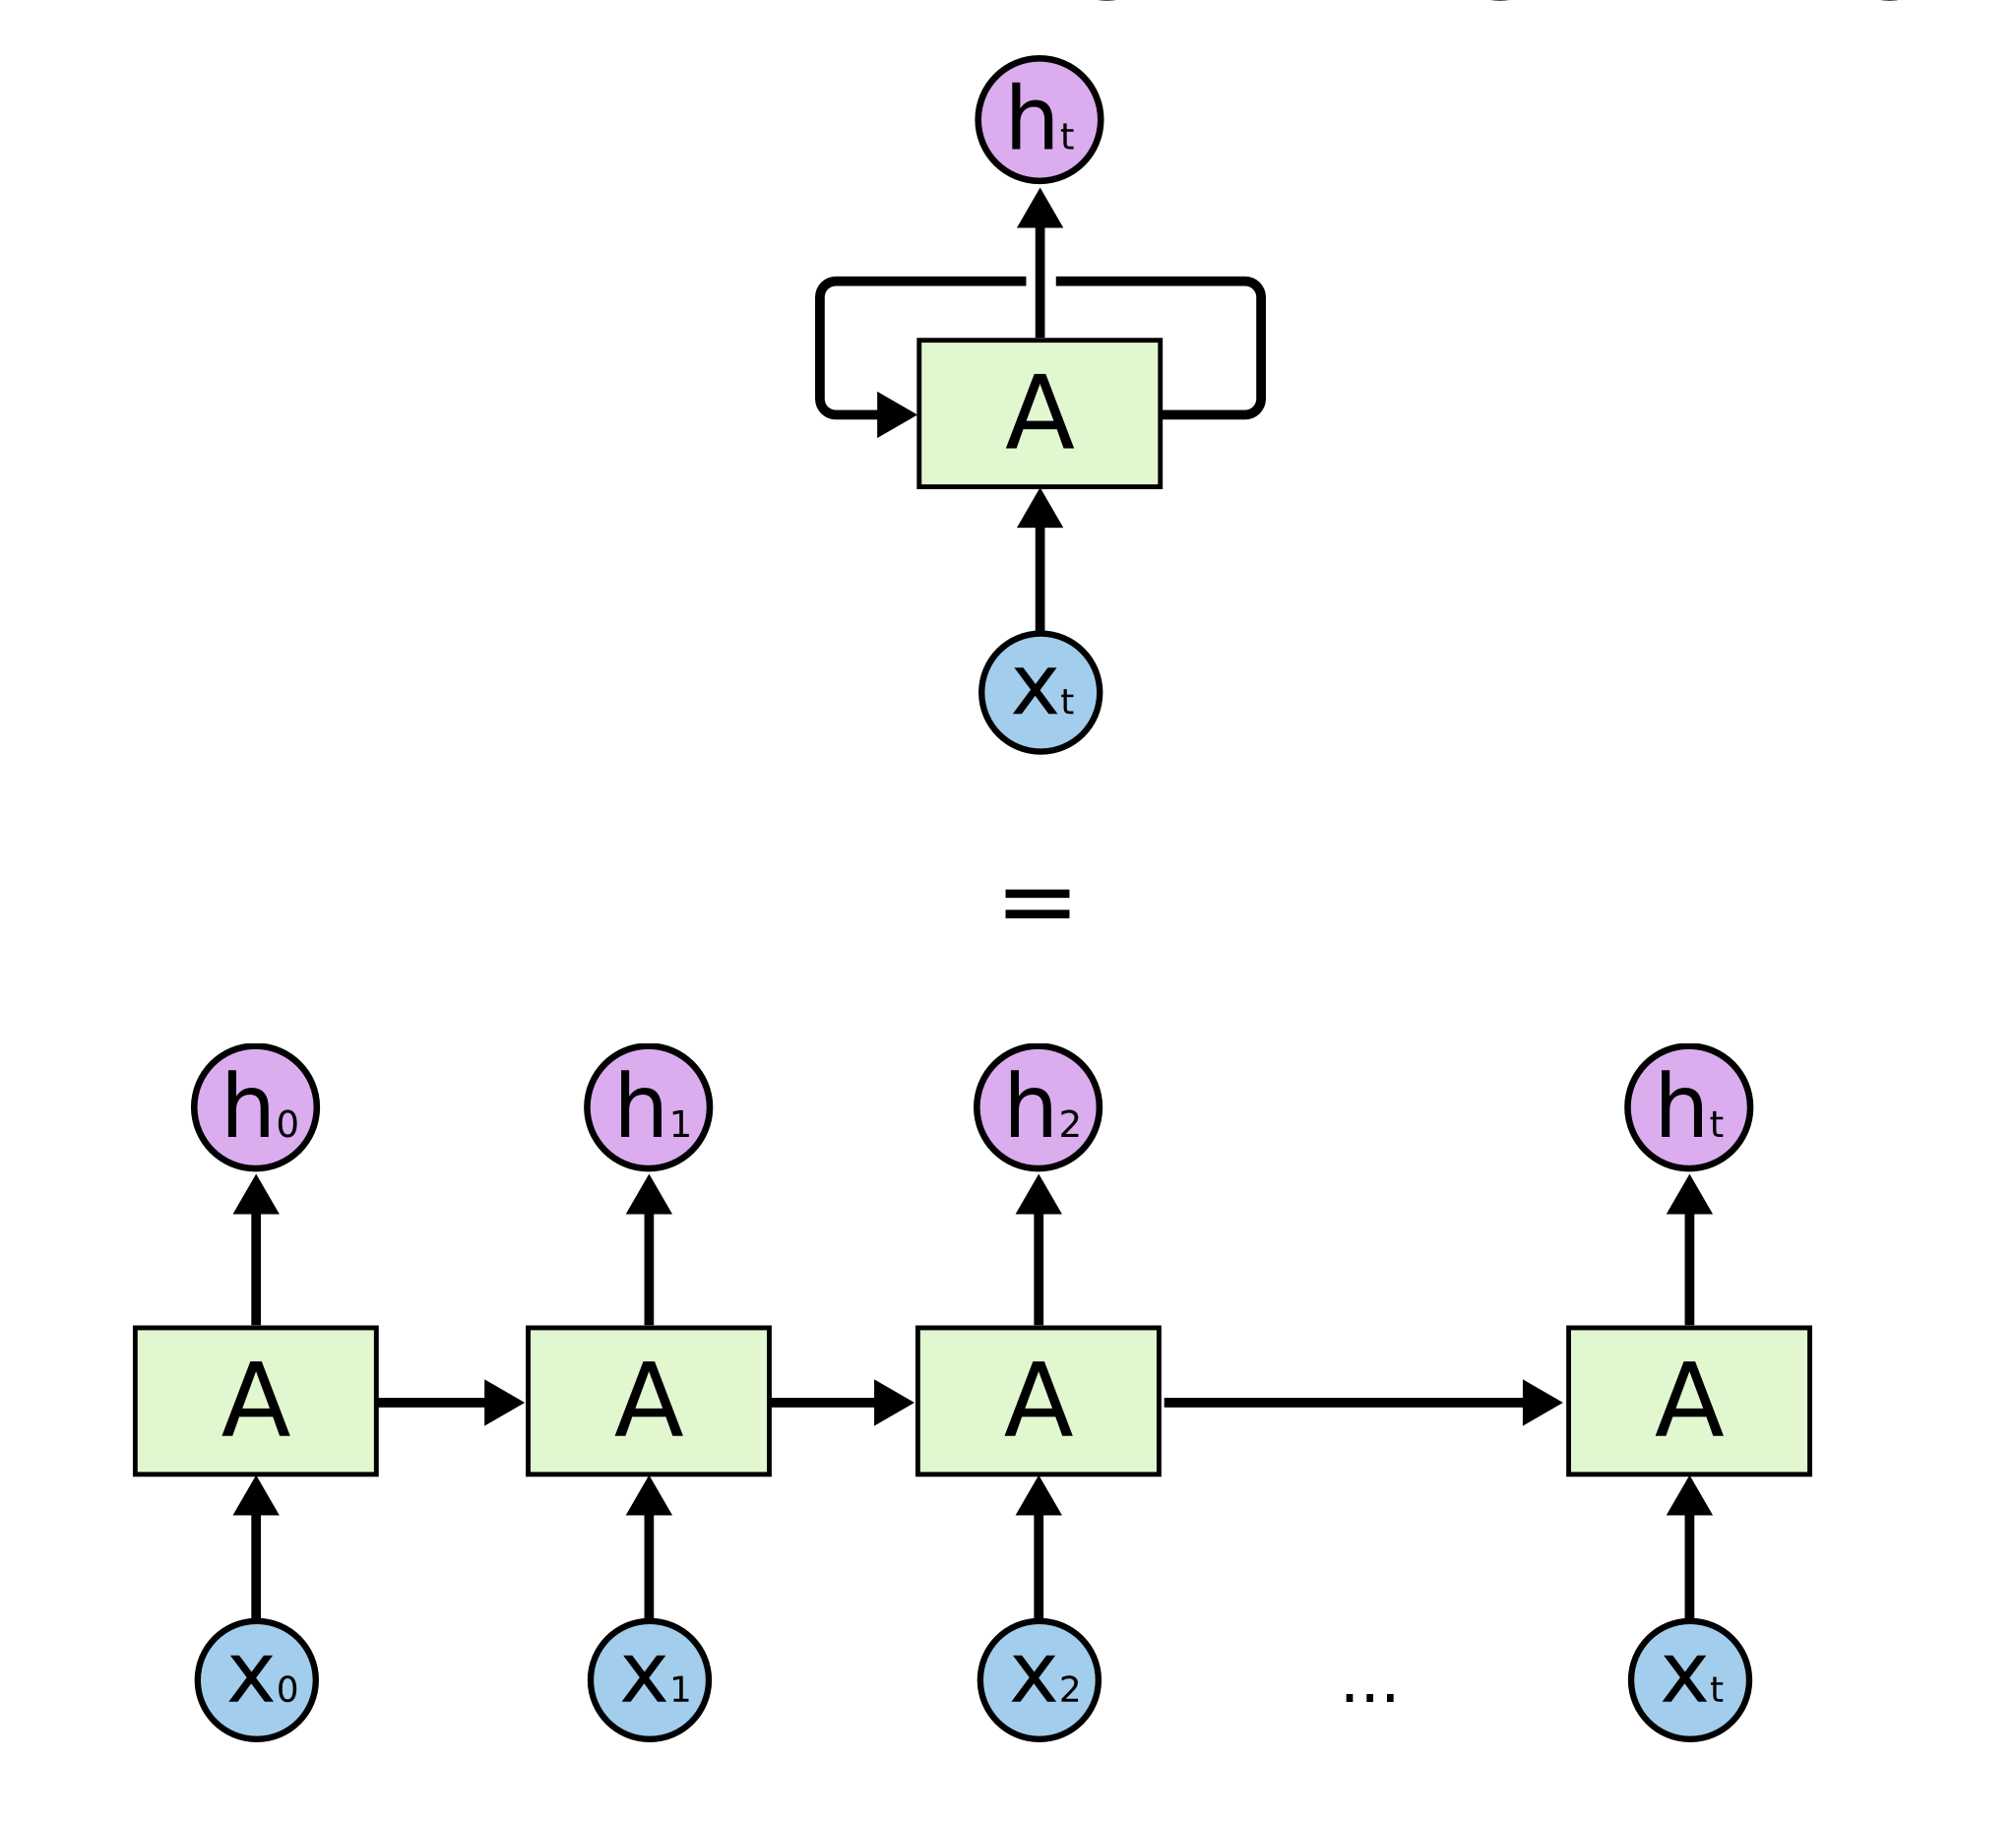
\includegraphics[scale=0.15]{RNN-unrolled} 
\caption{Recurrent Neural Network}
\label{fig.1}
\end{center}
\end{figure}

\subsection{Improvement in language understanding and generation}
Tellex et al.\cite{tellex2011understanding} proposed a framework that is able to instantiate a probabilistic graphical model dynamically from a natural language command, then does inference for events, tasks, objects, places and paths. Having that framework, a robotic system can learn to parse a complex command instead of hard-coded commands written by the developers. However, the proposed framework is still suffered from complicated linguistic phenomena such as negation ("\textbf{Don't} go to point A") or anaphora ("Pick the pallet and drop \textbf{it} at point B"). 

To address these challenge, Dukes et al. \cite{dukes2014semeval} introduced the Robot Commands Treebank of 3,394 spatial commands annotated with semantic information. Although the problem of spatial commands is a well-defined problem, the task is yet to solve completely because of the fact that natural language commands should be unconstrained and be composed by complex expressions with anaphora, ellipsis... These linguistic features are common in human daily language usage. Therefore, this treebank with a large amount of data models a wide range of linguistic aspects as multiword expressions, anaphoric references, ellipsis and negations in order to encourage researchers to work on machine learning approaches to solve input with more natural language.

Alongside with language understanding, natural language generation is also improved by the work of Seq2seq .\cite{sutskever2014sequence}. The authors used a multi-layered Long Short-Term Memory (LSTM) to map the input sequence to a vector of a fixed dimensionality, and then another deep LSTM to decode the target sequence from the vector. Not only having achieved good results in machine translation, this model was also applied in modelling conversation between computer and human by Vinyals et al. \cite{vinyals2015neural}. The model was trained on dialogue corpus (e.g. movie transcript dataset...) to generate response in an open-domain dialogue, not restricted to specific domains (e.g., booking an airline ticket) and does not require handcrafted rules.

\subsection{Improvement in cognitive modelling}
In "Human-Robot Interaction" \cite{feil2009human}, Feil-Seifer and Mataric mentioned one of the protruding challenges that is to build developmental robotics i.e. create intelligent machines that can learn from the world. Because  the  world  is  complex, it is  impossible  to  anticipate  every  single situation and  generate responses or rules in advance. Hence, it is important to develop robots with interactive learning, ability to learn new concepts incrementally without being re-programmed by professional programmers or Artificial Intelligence experts.

Unlike traditional machine learning methods, which learn from data, humans often learn from natural language instruction. Mimicking this ability, Azaria et al. \cite{azaria2016instructable} introduced an instructable intelligent personal agent named LIA. In the situation that there is a natural language command which LIA does not understand, it prompts the user to instruct a sequence of steps how to achieve the command, in natural language. To be able to learn new concepts, LIA makes use of a novel lexicon induction algorithm to generalize across taught commands by learning which words in the taught command correspond to each part of the complete logical form. The whole model was trained by scenarios generated by human on Amazon Mechanical Turk\footnote{https://www.mturk.com/}

In conclusion, the state-of-the-art research works discussed above have shown the key importance of learning when arming robotic system with NLP capability. Learning does not only significantly improve accuracy on each individual task, but open a new way for robots to approach and learn about the world.

\section{Ethical and performance concerns}
Although advances have been made, yet there are various concerns demanding to be solved when equipping robots with NLP for human-robot interaction, both in term of performance and ethical issues.

\subsection{Performance}
In the performance point of view, the question is mainly about whether the introduction of robotics and HRI provide effective and useful added value or not. For all the methods ranging from recognition, understanding to generation of language that we discussed in the previous sections, they were usually evaluated on the metrics of that specific task to show improvements. For examples, language generation in seq2seq\cite{sutskever2014sequence} was tested by BLEU (bilingual evaluation understudy) which is a common metric for translation and language generation task.

However, these intrinsic metrics are not enough to guarantee the desired social objectives to be successfully achieved by our robotic systems (e.g. response naturally and meaningfully to users, or entertaining their users). Therefore, the question about performance should be answered by a user's judgement. This kind of evaluation was also described as the last of Norman's seven stages of interaction \cite{norman1986cognitive}. When it comes to the evaluation of the outcome - the user has to compare the system state (as perceived by him/her) to the expected outcome and to decide if progress is being made or not.

In addition, there is also a raising concern that if the robot is actually assisting the user when we are too focused on a single mean of communication. For example, does a robot equipped with speech recognition and speech synthesis can understand people with speech disabilities? To address this issue, robots are not only equipped with one linguistic modal but several. For instance, ASIMO can perform and understand sign language alongside with speech. WLAS system \cite{azaria2016instructable} can read human lips and is able to translate to text so that robot can listen to human's speech better than humans themselves in noisy environment or underwater.

In regards to the noisy environment mentioned above, it is reasonable to show our concern about the adaptation of HRI systems developed in labs to be scalable to real-world scenarios with higher uncertainty. However, in my point of view, this is one of the most important reasons for researchers like Dukes et al. to introduce dataset with complicated phenomena trying to simulate near real-world environment and encouraged methods that can learn and adapt by both machine learning, deep learning and, in a different perspective, interactive learning (which is also able to be implemented by reinforcement learning, a branch of machine learning).

The last issue we will discuss in this section is the robot's level of autonomy. In my opinion, this totally depends on the design of the robot to suit with its specific task. Whether it leaves space for ultimate authority to be assigned to the user to take control over or not is decided by the system designers. One trivial implementation of the signal from user is the emergency red button. This mechanism can be also implemented on HRI system with NLP by a "code word", which word when being pronounced by user will stop all creative responses and will trigger robot to follow a pre-coded steps.

\subsection{Ethical issues}
Not only performance, when deploying robotic systems with regard to NLP-equipped HRI, ethical issues need to be kept in mind with equal importance. The first issue, obviously, should be the concern of safety. Is the robot safe in use, and does it enhance safety for its users? Through the lens of NLP, the safety of language generation by robots should be investigated to answer this question: are the generated responses contain bad words, hate speech or racist materials. This is not a nonsense anxiety as this kind of incident has happened with Tay, a Microsoft's Twitter\footnote{https://twitter.com/} bot\footnote{https://www.theverge.com/2016/3/24/11297050/tay-microsoft-chatbot-racist} that learned racism and hate speech by interacting with other Twitter users (an implementation of interactive learning) within 24 hours after having been deployed.

The second ethical issue concerns about the need of an imitation that is as close as possible to human behaviours. This is one of the methods to pass the Turing Test, which is one milestone to come up with a general artificial intelligence. However, the Uncanny Valley Theory\cite{mori2012uncanny} states that as a robot starts approximating a human very closely but not perfectly, users may respond with revulsion. This can be explain by a hypothesis of human nature to protect themselves from dangerous situation by a sense that "something is not quite right". In other words, anthropomorphism can be viewed negatively if the actions of the robot do not meet the user's expectations. One example from our discussed state-of-the-art robots is Sophia from Hanson robotics, which fully resembles  human face, smile and facial expressions. However, it was reported to be scary from the public opinion\footnote{https://www.cnet.com/news/crazy-eyed-robot-wants-a-family-and-to-destroy-all-humans/} , while Moro, Kuri and other robots with the same ability to conduct conversation, yet without human appearance, were conceived as more friendly and approachable.

The last problem involves with social effects of robotics and HRI. Does it affect negatively or positively the social interaction between humans in the community? This question is yet to be fully answered. Although there is a clear concern of human-computer interaction, especially human-mobile, that affects negatively in daily social interaction, it is too soon to conclude about the polarity of HRI effect. There are two reasons for this. First, robotics and HRI are not popular among our population in compare to computers and mobile phones, hence, no persuasive and alarming conclusion can be drawn. Second, NLP equipped in robotic system is expected to promote natural communication between human and robot. Therefore, it should increase the amount of natural interaction, not to decrease it, yet has not been scientifically proven.

In addition to the social effect, equipping NLP and artificial intelligence in robotic systems creates a fear of exclusive communication among robots themselves, leads to the conspiracy of human losing control and robot-related apocalypse. However, this should be the least problematic one, in my opinion. In fact, intermediate language invented by robots were observed and recorded, from Lingodroids\cite{schulz2010robots}\footnote{https://www.youtube.com/watch?v=7u9OvtEkd1A} to seq2seq. Nevertheless, this is expected phenomenon that robots create a kind of jargon vocabulary/encoding to efficiently communicate with one another. Through this observation, we can learn and form hypothesis about how our natural languages have evolved over time. Moreover, the level of intelligence of our current system is still far from the point that we can start being concerned about a war between humankind and robots. Let us get to that point first.

\section{Roles of humans in typical applications of human-robot interaction}
Scholtz, in "Theory and evaluation of HRIs", (2003)\cite{scholtz2003theory}, introduced a categorisation of roles that humans typically play in HRI applications. This categorisation is an expanded version from the version in Scholtz and Jean (2002)\cite{scholtz2002human} with three roles:  supervisor, operator, and peer. Mechanic is added in and peer is finely separated into teammate and bystander as follows:
\begin{itemize}
	\item Supervisor, in which humans have to take controlling the overall situation by monitoring and evaluating robots' actions.
	\item Operator, when a human fine-tunes several parameters in the robot's control mechanism in order to prevent abnormal behaviour to happen again or to alter a designated behaviour to  a more appropriate one; or even to take over and manually operate the robot in some specific circumstances.
	\item Mechanic, is to deal with physical interventions by adjusting or fixing physical components of the robot.
	\item Teammate: collaborates with the robot to perform a task as demonstrated in Lego rocket assembly task by Vogt et al. in which human and robot simultaneously assemble two separated rocket parts (one hold by a human, the other hold by robot arm)\footnote{https://www.youtube.com/watch?v=3pAYpprFx8Y}.
	\item Bystander: function of a bystander can be part of the robot working environment (e.g. robot might avoid bystanders to avoid collision) or to observe robot's behaviours for further analysing of robot's actions without explicit interaction with the robot.
\end{itemize}

It is important to note that Scholtz categorised human's roles in the perspective of human. In contrast, Goodrich et al. (2007)\cite{goodrich2007human} proposed the following additional roles of human in the robot's point of view, i.e. the robot plays a more active roles:
\begin{itemize}
	\item Mentee: a robot is in a teaching or leadership role with respect to a human, hence, human is to be mentee while robot is the mentor. This is an important role of robots yet emerging with educational robots like NAO that we discussed in the first section or robots that work in rehabilitation centres. These robots either guide or encourage humans to follow a series of steps that lead them to achieve a goal, either learn something new or to recover from stroke\footnote{https://www.youtube.com/watch?v=DEd9ci-qLzk}.
	\item Information Consumer: the robot notifies the human by collecting information, especially from hazardous environments or disasters (e.g. reconnaissance tasks such as drone or search-and-rescue robot...)
\end{itemize}

\section{Conclusion}

In conclusion, the report has discussed some main aspects of the huge area of applying NLP in robotics study. State-of-the-art robots were collected and compared by their functions, especially natural language capability. The report also proved that learning is crucial by reviewing state-of-the-art research work and summarised main points of each work.  Ethical and performance issues were also discussed with author's opinion and proofs from literatures following by a brief review of human's roles in HRI. Although having tried to cover crucial points of this joint-discipline field with state-of-the-art works, the report is clearly limited and expected to be outdated with the incredible speed of researchers working in the study of robotics and artificial intelligence, in which the progress is measured by months. However, this is a good sign that our knowledge in the field is improved and strengthened day by day.


\section{Acknowledgements}

I would like to thank Prof. Simon G. Fabri and Dr. Marvin K. Bugeja for their inspiration, knowledge and constructive feedbacks during our "Human-robot interaction: speech and beyond" unit in the course "LIN5508: Language and Embodied Agents", which lead to my decision to work on this topic. I am also appreciated of the ideas from Dr. Andrea De Marco, Prof. Patrizia Paggio and Prof. Catherine Pelachaud in the same course that broadened my limited mind and understanding.

%\nocite{*}

\bibliographystyle{lrec2014}
\bibliography{main}

\end{document}













